\section{BaM}
\label{sec:chapter_4_section_1}
Il Progetto BaM (Building and Modelling) sviluppato in collaborazione con il CNG (Comitato Nazionale Geometri),
nasce dall'idea di far realizzare, agli studendi frequentanti le scuole medie in Italia,
``\emph{l'aula che vorrei}''. Lo scopo principale di questa iniziativa \'e sensibilizzare gli studenti a utilizzare
materiali ecosostenibili e rispettare l'ambiente.
Gli alunni avranno poi la possibilità di scegliere degli elementi con cui personalizzare l’aula virtuale.
La lista degli oggetti 3D presenti in libreria ha l’obiettivo di far sperimentare l’uso di uno strumento di progettazione
e di rappresentazione della realtà e di dare spunti su alcune tematiche.\\
\\Per questo motivo il software è stato strutturato in modo che a ogni elemento è associato un punteggio su:
\begin{itemize}
\item impatto Ecologico;
\item impatto Energetico;
\item sicurezza;
\item rispetto della diversità/disabilità;
\end{itemize}
Vincerà il team che realizzerà la classe con il punteggio più alto, risultante dalla somma dei materiali scelti
tra quelli presenti in libreria. Per ottenere un punteggio alto, bisogna rispettare i principi delle
“3E” (Edilizia – Energia - Economia) e delle “3R” (Ridurre, Riutilizzare, Riciclare)!. Vediamo un esempio
di modellazione di aula
\begin{figure}[htbp] %  figure placement: here, top, bottom, or page
   \centering
   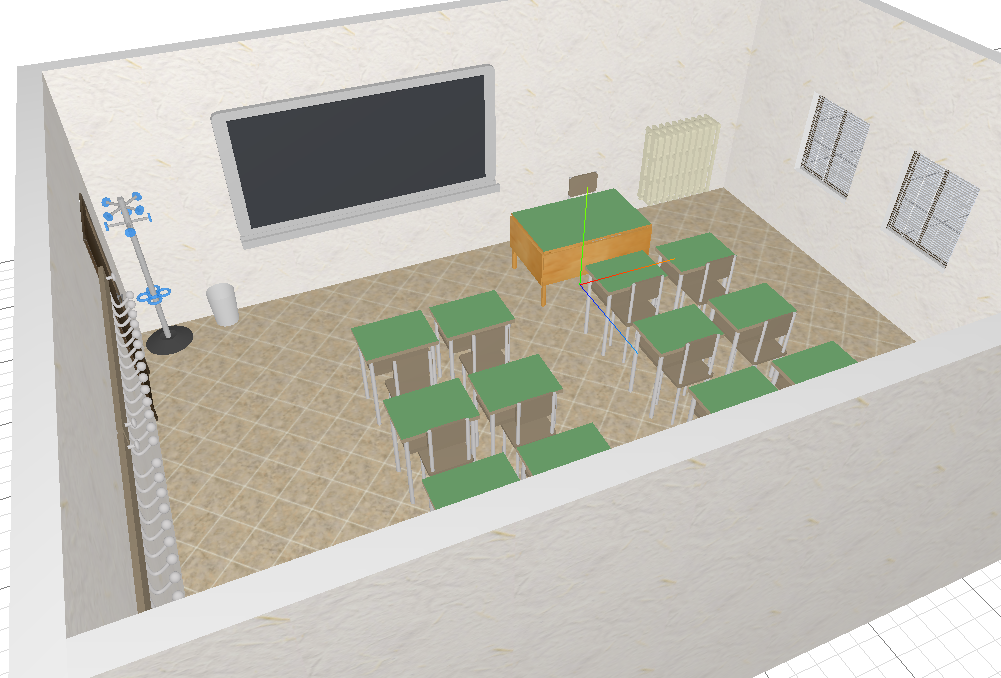
\includegraphics[width=1\linewidth]{images/3d-school-2}
   \caption{Vista 3D modello aula}
   \label{fig:revit}
   \end{figure}

\newpage

I plugins presenti all'interno del catalogo, sono stati suddivisi in categorie, per consentire una valutazione al
termine dell'esperienza di modellazione dell'aula.
Il primo gruppo di plugins riportato sono (come si evince dalla Figura~\ref{fig:figura1}): un appendiabiti, un armadietto,
un attaccapanni ed un porta ombrelli.\\

\begin{figure}[htbp]
\begin{center}
\begin{tabular}{c @{\hspace{1em}} c}
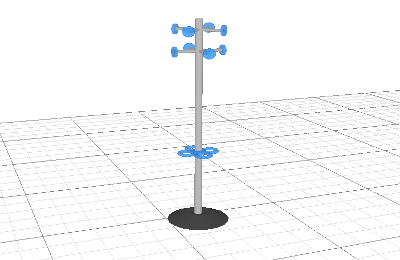
\includegraphics[width=5.5cm]{images/hanger} &
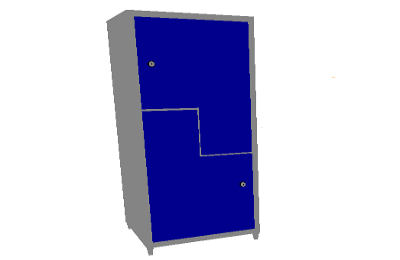
\includegraphics[width=5.5cm]{images/wardrobe} \\
 (a) & (b) \\
\end{tabular}
\begin{tabular}{c @{\hspace{1em}} c}
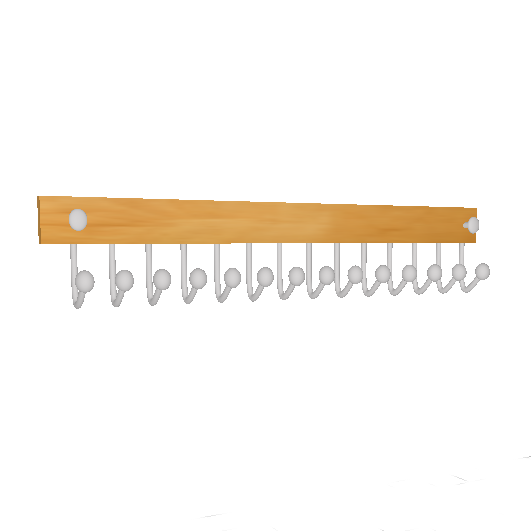
\includegraphics[width=5.5cm]{images/attaccapanni2} &
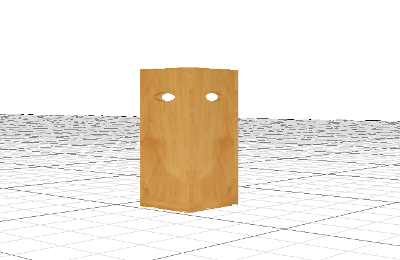
\includegraphics[width=5.5cm]{images/portaombrelli} \\
 (c) & (d) \\
\end{tabular}
\end{center}
\caption{Dettaglio Plugins: (a) appendiabiti, (b) armadietto, (c) attaccapanni, (d) portaombrelli}\label{fig:figura1}
\end{figure}
\newpage

Il secondo gruppo di plugins riportato sono (come si evince dalla Figura~\ref{fig:figura2}): un banco, una cattedra,
una lavagna ed una lavagna interattiva multimediale.\\

\begin{figure}[htbp]
\begin{center}
\begin{tabular}{c @{\hspace{1em}} c}
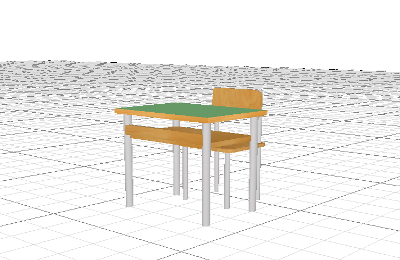
\includegraphics[width=5.5cm]{images/banco2} &
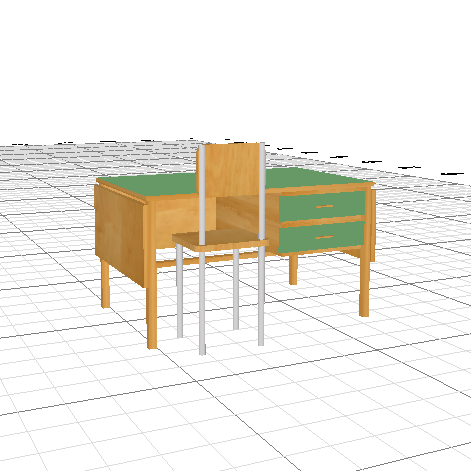
\includegraphics[width=5.5cm]{images/cattedra2} \\
 (a) & (b) \\
\end{tabular}
\begin{tabular}{c @{\hspace{1em}} c}
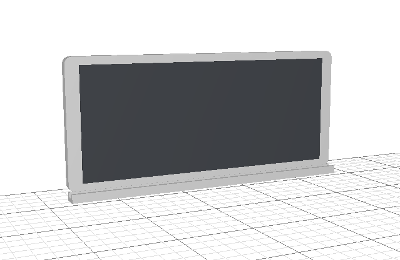
\includegraphics[width=5.5cm]{images/lavagna} &

\includegraphics[width=5.5cm]{images/lim} \\
 (c) & (d) \\
\end{tabular}
\end{center}
\caption{Dettaglio Plugins: (a) banco, (b) cattedra, (c) lavagna, (d) lim}\label{fig:figura2}
\end{figure}
\newpage

Il terzo gruppo di plugins riportato sono (come si evince dalla Figura~\ref{fig:figura3}): un cestino, gruppo di cestini
per la raccolta differenziata, un condizionatore d'aria ed termosifone.\\


\begin{figure}[htbp]
\begin{center}
\begin{tabular}{c @{\hspace{1em}} c}
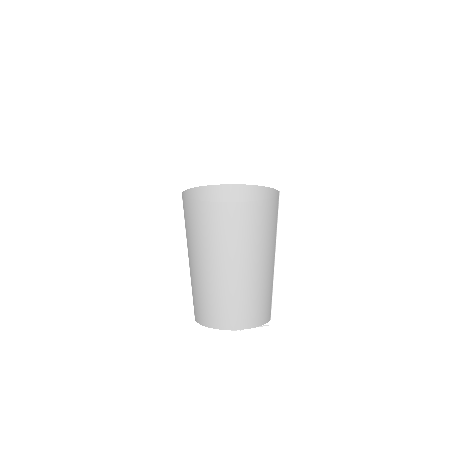
\includegraphics[width=5.5cm]{images/cestino} &
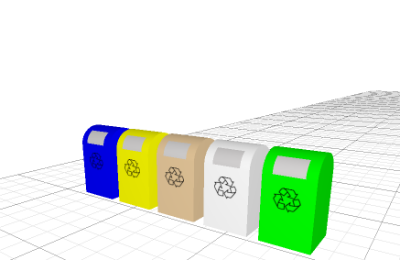
\includegraphics[width=5.5cm]{images/recycling-bins} \\
 (a) & (b) \\
\end{tabular}
\begin{tabular}{c @{\hspace{1em}} c}
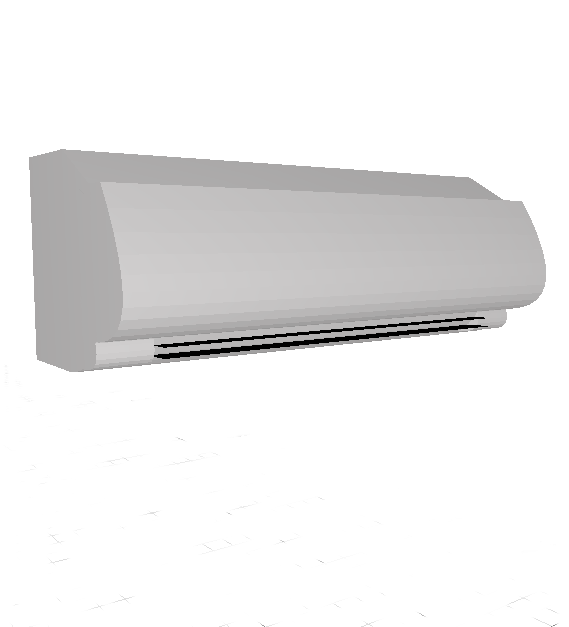
\includegraphics[width=5.5cm]{images/condizionatore} &
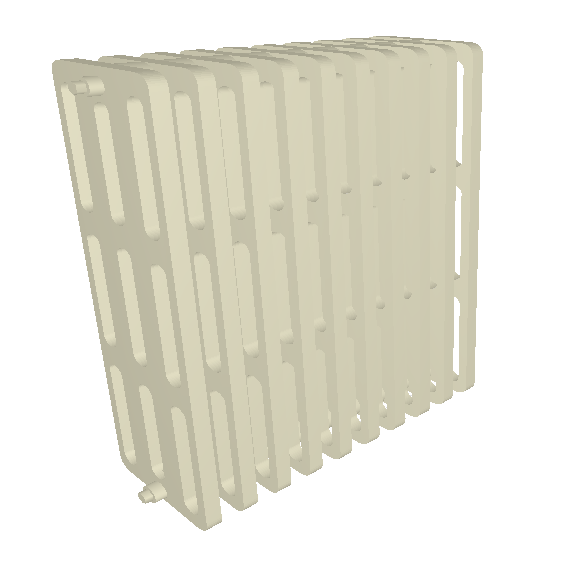
\includegraphics[width=5.5cm]{images/termosifone} \\
 (c) & (d) \\
\end{tabular}
\end{center}
\caption{Dettaglio Plugins: (a) cestino, (b) cestini differenziata, (c) condizionatore, (d) termosifone}\label{fig:figura3}
\end{figure}
\newpage

Il terzo gruppo di plugins riportato sono (come si evince dalla Figura~\ref{fig:figura4}): una libreria, un computer,
una finestra con tenda ed una con veneziana.\\

\begin{figure}[htbp]
\begin{center}
\begin{tabular}{c @{\hspace{1em}} c}
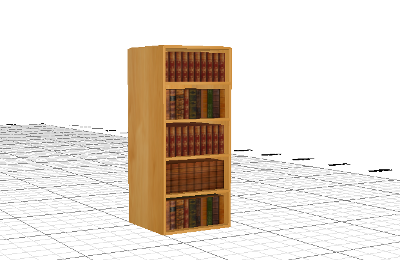
\includegraphics[width=5.5cm]{images/bookcase} &
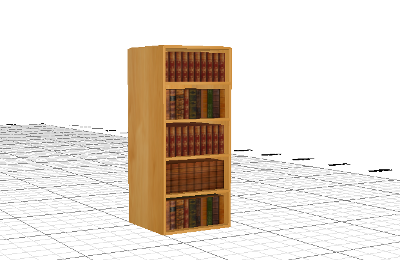
\includegraphics[width=5.5cm]{images/bookcase} \\
 (a) & (b) \\
\end{tabular}
\begin{tabular}{c @{\hspace{1em}} c}
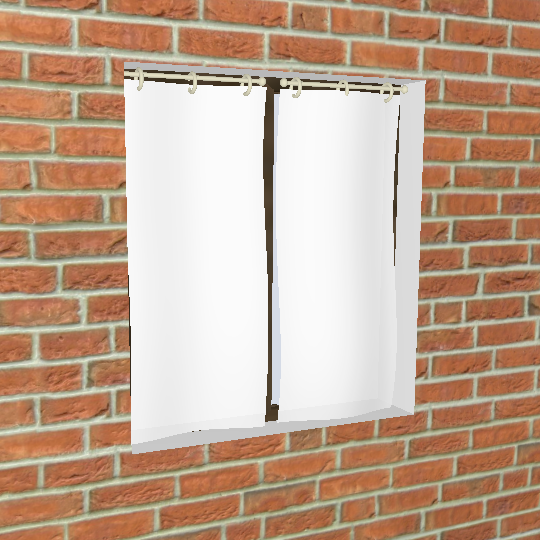
\includegraphics[width=5.5cm]{images/tenda} &
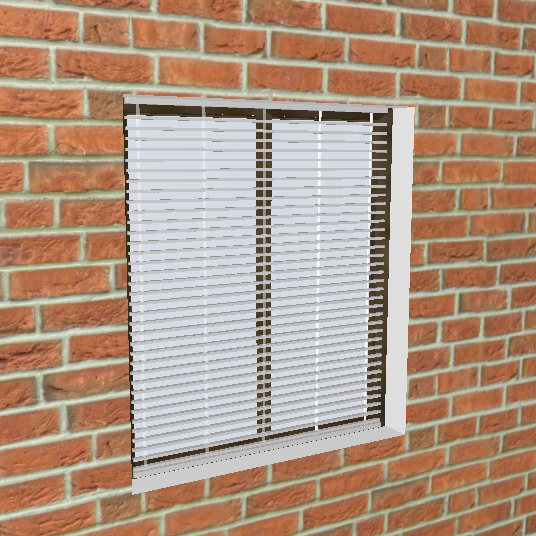
\includegraphics[width=5.5cm]{images/veneziana} \\
 (c) & (d) \\
\end{tabular}
\end{center}
\caption{Dettaglio Plugins: (a) libreria, (b) ???, (c) finestra con tenda, (d) finestra con veneziana}\label{fig:figura4}
\end{figure}

\newpage
